\chapter{La derivada de Malliavin}

\section{Definición \guia{Definición 7.1}}
Sea $\mathcal S$ la clase de variables suaves $F=f(W(h_1),\dots,W(h_n))$ con
$f\in C_p^\infty(\R^n)$. Se define
\[
  \D_tF=\sum_{i=1}^n \partial_i f(W(h_1),\dots,W(h_n))\,h_i(t).
\]
$\D$ es cerrable de $L^2(\Omega)$ en $L^2(\Omega;\Hil)$; $\Dom$ es la clausura de
$\mathcal S$ para la norma $\norm{F}^2_{1,2}=\E[F^2]+\E\norm{\D F}^2_\Hil$.

\paragraph{Interpretación direccional.} Para $h\in\Hil$,
\[
  \ip{\D F}{h}=\lim_{\varepsilon\to0}\frac1\varepsilon\Big[F\big(\omega+\varepsilon\textstyle\int_0^\cdot h\big)-F(\omega)\Big],
\]
es decir, $\D F$ es el gradiente de $F$ en las direcciones de Cameron--Martin.

\section{Reglas de cálculo}
\begin{itemize}
  \item \textbf{Regla de la cadena:} $\D\,\varphi(F)=\varphi'(F)\D F$ para $\varphi\in C^1_b$
        (y para $\varphi$ Lipschitz con $\varphi'$ débil).
  \item \textbf{Caos:} $\D_t I_n(f_n)=n I_{n-1}(f_n(\cdot,t))$; por tanto
        $F\in\Dom \iff \sum_n n\,n!\norm{f_n}^2<\infty$.
  \item \textbf{Adaptación:} si $F$ es $\F_s$-medible, $\D_tF=0$ para $t>s$.
\end{itemize}

\section{Ejemplos}
\begin{center}
\begin{tabular}{ll}
  $F$ & $\D_tF$, \ $t\in[0,T]$\\\hline
  $W_T^p$ & $pW_T^{p-1}$\\
  $\int_0^T W_s\dd s$ & $T-t$\\
  $\max_{s\le T}W_s$ & $\ind_{[0,\tau^*]}(t)$, \ $\tau^*=\arg\max$ \guia{Prop.~7.16}\\
  $S_T=S_0e^{(r-\sigma^2/2)T+\sigma W_T}$ & $\sigma S_T$\\
  $\int_0^T S_u\dd u$ & $\sigma\int_t^T S_u\dd u$\\
\end{tabular}
\end{center}

\section{Versión discreta}
Si $F=\phi(\Delta W_0,\dots,\Delta W_{n-1})$ sobre una malla $t_k=kT/n$, entonces
$\D_tF=\partial\phi/\partial(\Delta W_k)$ para $t\in[t_k,t_{k+1})$. Esta es la
aproximación que implementa \codigo{derivative.discrete\_malliavin\_derivative}.

\begin{figure}[h]
  \centering
  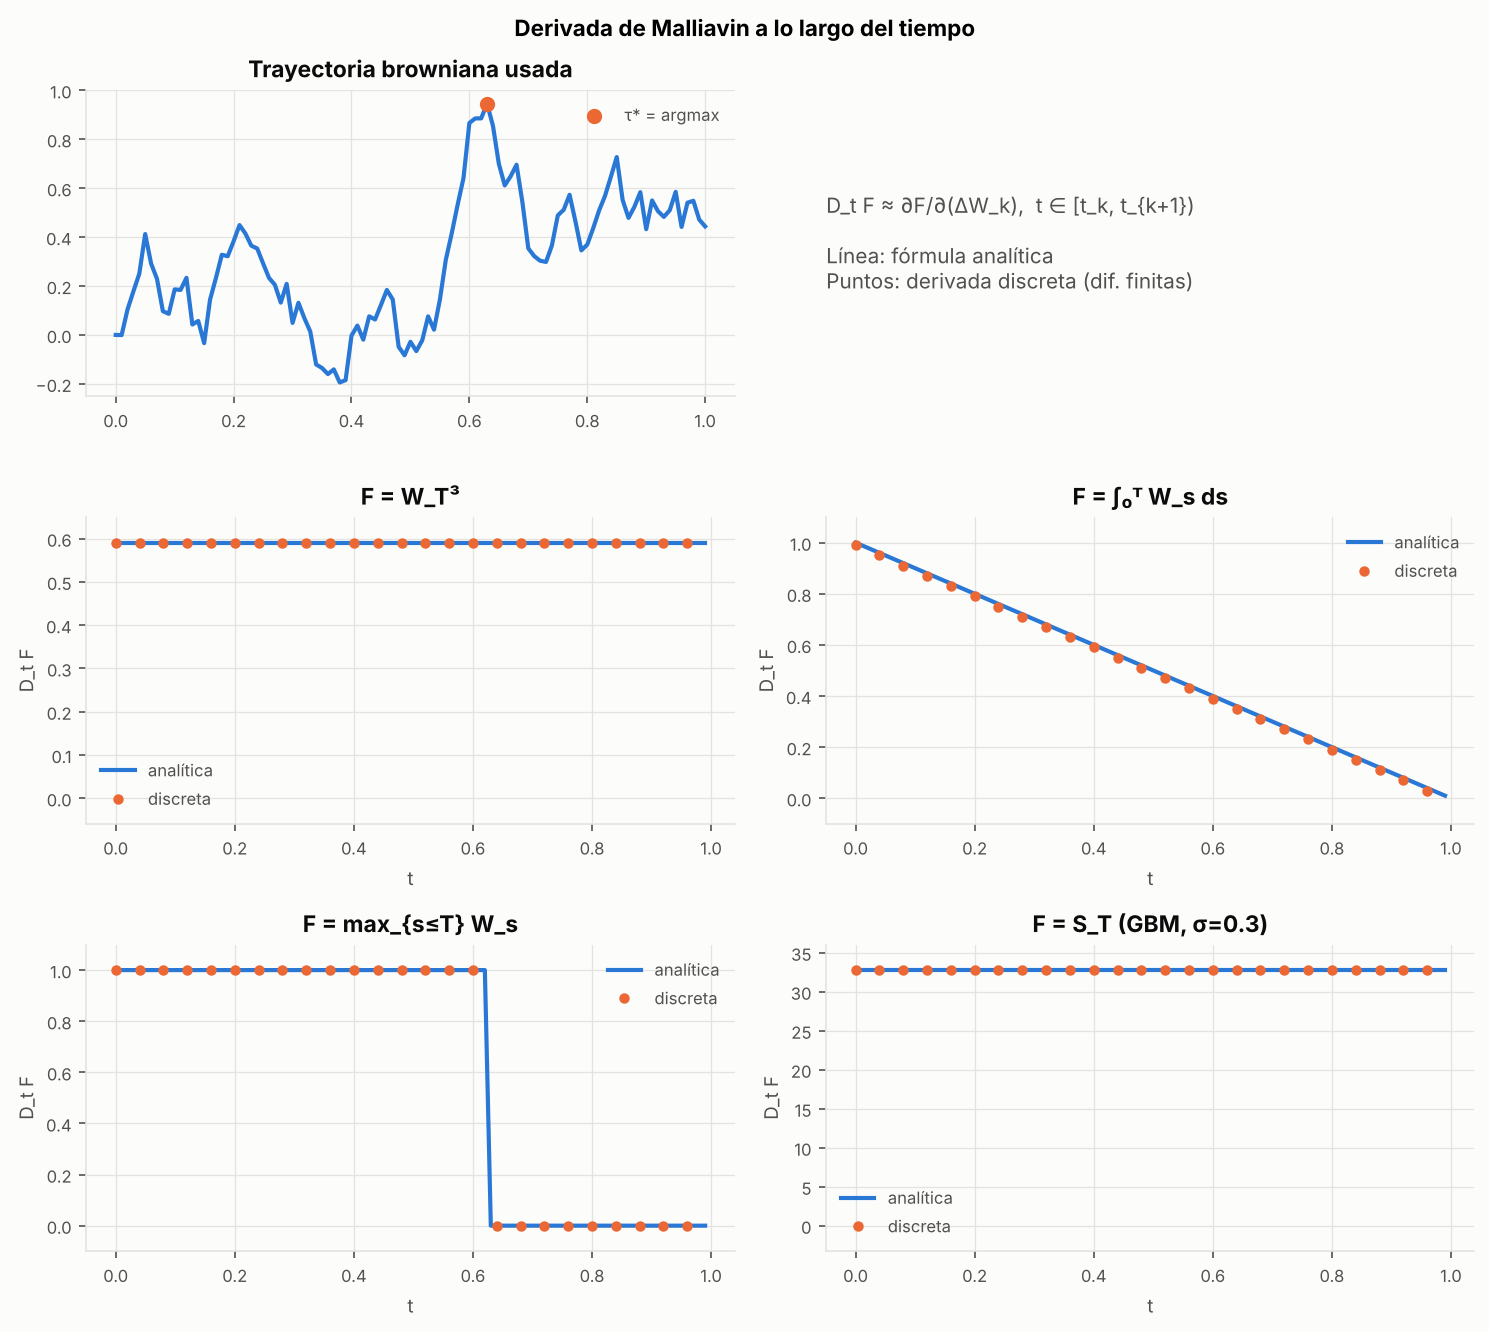
\includegraphics[width=0.9\linewidth]{02_derivada_malliavin}
  \caption{Derivada discreta frente a la analítica (\codigo{examples/02\_derivada\_malliavin.py}).}
\end{figure}
